%!TEX root = hulk.tex
%!TeX TS-program = pdflatex
%!TeX encoding = UTF-8 Unicode
%!TeX spellcheck = en-US
%!BIB TS-program = biber
% -*- coding: UTF-8; -*-
% vim: set fenc=utf-8
% Guidelines for Writing a Good NIPS Paper : https://nips.cc/Conferences/2015/PaperInformation/EvaluationCriteria
% https://github.com/bicv/Perrinet2015BICV_sparse/blob/master/sparse.tex
%%%%%%%%%%%%%%%%%%%%%%%%%%%%%%%%%%%%%%%%%%%%%%%%%%%%%%%%%%%%%%%%%%%%%
\def\Draft{0}%
\def\Draft{1}%
%%%%%%%%%%%%%%%%%%%%%%%%%%%%%%%%%%%%%%%%%%%%%%%%%%%%%%%%%%%%%%%%%%%%%
\if 1\Draft
\documentclass[a4paper, 11pt, draft]{article} % For LaTeX2e
\else
\documentclass[a4paper, 11pt]{article} % For LaTeX2e
\fi
% if you need to pass options to natbib, use, e.g.:
% \PassOptionsToPackage{numbers, compress}{natbib}
% before loading nips_2017
%
% to avoid loading the natbib package, add option nonatbib:
\usepackage[nonatbib]{nips_2018}
%\usepackage{nips_2018}
%\usepackage[final]{nips_2018}
%
%============ common ===================
%\usepackage[utf8]{luainputenc}
%\usepackage[english]{babel}%
%%\usepackage{csquotes}%
%\usepackage[autostyle]{csquotes}
%%% Sans-serif Arial-like fonts
%\renewcommand{\rmdefault}{phv}
%\renewcommand{\sfdefault}{phv}
%   \usepackage{textcomp}
%   \usepackage{libertine}%[sb]
%   \usepackage[varqu,varl]{inconsolata}% sans serif typewriter
%   \usepackage[libertine,bigdelims,vvarbb]{newtxmath} % bb from STIX
%   \usepackage[cal=boondoxo]{mathalfa} % mathcal
%%   \useosf % osf for text, not math
%   \usepackage[supstfm=libertinesups,%
%    supscaled=1.2,%
%    raised=-.13em]{superiors}
%\usepackage[utf8]{inputenc} % allow utf-8 input
%\usepackage[T1]{fontenc}    % use 8-bit T1 fonts
%\usepackage{dsfont}
%\usepackage{hyperref}       % hyperlinks
% --------------------------------------------------------------------------
%                    METADATA
% --------------------------------------------------------------------------
\newcommand{\AuthorA}{Boutin}%
\newcommand{\FirstNameA}{Victor}%
\newcommand{\AuthorB}{Franciosini}%
\newcommand{\FirstNameB}{Angelo}%
\newcommand{\AuthorC}{Perrinet}%
\newcommand{\FirstNameC}{Laurent U}%
\newcommand{\Institute}{Institut Neurosciences Timone, Marseille, France}%\\ Aix Marseille Univ, CNRS}%
\newcommand{\Organism}{Aix Marseille Universit\'e, CNRS}%
\newcommand{\Address}{27, Bd. Jean Moulin, 13385 Marseille Cedex 5, France}%
\newcommand{\Website}{http://invibe.net/LaurentPerrinet}%
\newcommand{\EmailA}{victor.boutin@univ-amu.fr}%
\newcommand{\EmailB}{angelo.franciosini@univ-amu.fr}%
\newcommand{\EmailC}{laurent.perrinet@univ-amu.fr}%
\newcommand{\WebsiteC}{http://invibe.net/LaurentPerrinet}%
\newcommand{\Title}{%
%A fast algorithm for unsupervised learning
An adaptive algorithm for unsupervised learning
%alternatives: - Homeostasis is necessary for the unsupervised learning of orientation-selective cells
%# Homeostatic Unsupervised Learning of Kernels
}%
\newcommand{\Abstract}{
The formation of structure in the brain, that is, of the connection between cells within neural populations, is by large an unsupervised learning process: The emergence of this architecture is mostly self-organized. In the primary visual cortex of mammals, for example, one may observe during development the emergence of cells selective to localized, oriented features. This leads to the development of a rough representation of contours of the retinal image in area V1.
We modeled these representations using sparse unsupervised learning algorithms.
These algorithms alternate a coding phase to encode the information with a learning phase to find the proper encoder. A major difficulty faced by these types of algorithms is to deduce good representation while  knowing immature encoders, and to learn good encoders with a non-optimal representation
To address this problem, we propose here to introduce a new regulation process between learning and coding, called homeostasis. Our homeostasis is compatible with a neuro-mimetic architecture and allows for the fast emergence of localized filters sensitive to orientation. 
The key to this algorithm lies in a simple adaptation mechanism based on non-linear functions that reconciles the antagonistic processes that occur at the coding and learning time scales.
We tested this unsupervised algorithm with this homeostasis rule for a range of existing unsupervised learning algorithms coupled with different neural coding algorithms. In addition, we propose a simplification of this optimal homeostasis rule by implementing a simple heuristic on the probability of activation of neurons. Compared to the optimal homeostasis rule, we show that this heuristic allows to implement an even faster unsupervised learning algorithm while keeping a large part of its effectiveness. These results demonstrate the potential application of such a strategy to the fast classification of images, for example in hierarchical and dynamic architectures.
}
\newcommand{\Keywords}{Vision, Sparseness, Computer vision, Unsupervised learning, Neuroscience}%
\newcommand{\Acknowledgments}{%
%This work was supported by XXXAFXXX and the Doc2Amu project which received funding from a co-fund with the European Union's Horizon 2020 research and innovation programme and the region Provence Alpes Cote d'Azur. 
%
This research has received funding from the European Union’s Horizon 2020 research and innovation programme under the Marie Skłodowska-Curie grant agreement No713750. Also, it has been carried out with the financial support of the Regional Council of Provence-Alpes-Côte d’Azur and with the financial support of the A*MIDEX (n° ANR- 11-IDEX-0001-02), funded by the Investissements d'Avenir project funded by the French Government, managed by the French National Research Agency (ANR).
}
\newcommand{\Links}{%
\begin{itemize}
\item Correspondence and requests for materials should be addressed to LUP (email:\EmailC ).
\item Code and supplementary material available at \url{\WebsiteC/Publications/BoutinFranciosiniPerrinet18hulk}.
\end{itemize}
} %
\usepackage{filecontents}
% --------------------------------------------------------------------------
% --------------------------------------------------------------------------
% --------------------------------------------------------------------------
\begin{filecontents}{hulk.bib}

@ARTICLE{Kingma13,
   author = {{Kingma}, D.~P and {Welling}, M.},
    title = "{Auto-Encoding Variational Bayes}",
  journal = {ArXiv e-prints},
archivePrefix = "arXiv",
   eprint = {1312.6114},
 primaryClass = "stat.ML",
 keywords = {Statistics - Machine Learning, Computer Science - Learning},
     year = 2013,
    month = dec,
   adsurl = {http://adsabs.harvard.edu/abs/2013arXiv1312.6114K},
}


@article{Doersch2016,
	Abstract = {In just three years, Variational Autoencoders (VAEs) have emerged as one of the most popular approaches to unsupervised learning of complicated distributions. VAEs are appealing because they are built on top of standard function approximators (neural networks), and can be trained with stochastic gradient descent. VAEs have already shown promise in generating many kinds of complicated data, including handwritten digits, faces, house numbers, CIFAR images, physical models of scenes, segmentation, and predicting the future from static images. This tutorial introduces the intuitions behind VAEs, explains the mathematics behind them, and describes some empirical behavior. No prior knowledge of variational Bayesian methods is assumed.},
	Author = {Doersch, Carl},
	Journal = {arXiv:1606.05908 [cs, stat]},
	Keywords = {Computer Science - Learning, Statistics - Machine Learning},
	Month = jun,
	Title = {Tutorial on Variational Autoencoders},
	Url = {http://arxiv.org/abs/1606.05908},
	Year = {2016},}

@article{Eichhorn09,
  title={Natural image coding in V1: how much use is orientation selectivity?},
  author={Eichhorn, Jan and Sinz, Fabian and Bethge, Matthias},
  journal={PLoS computational biology},
  volume={5},
  number={4},
  pages={e1000336},
  year={2009},
  publisher={Public Library of Science}
}

@incollection{Zoran12,
	Author = {Zoran, Daniel and Weiss, Yair},
	Booktitle = {Advances in Neural Information Processing Systems 25},
	Editor = {F. Pereira and C. J. C. Burges and L. Bottou and K. Q. Weinberger},
	Pages = {1736--1744},
	Publisher = {Curran Associates, Inc.},
	Title = {Natural Images, Gaussian Mixtures and Dead Leaves},
	Url = {http://papers.nips.cc/paper/4758-natural-images-gaussian-mixtures-and-dead-leaves.pdf},
	Year = {2012},
	Bdsk-Url-1 = {http://papers.nips.cc/paper/4758-natural-images-gaussian-mixtures-and-dead-leaves.pdf}}

@article{Hansel12,
  title={The mechanism of orientation selectivity in primary visual cortex without a functional map},
  author={Hansel, David and van Vreeswijk, Carl},
  journal={Journal of Neuroscience},
  volume={32},
  number={12},
  pages={4049--4064},
  year={2012},
  publisher={Soc Neuroscience}
}

@article{Ringach02,
  title={Spatial structure and symmetry of simple-cell receptive fields in macaque primary visual cortex},
  author={Ringach, Dario L},
  journal={Journal of neurophysiology},
  volume={88},
  number={1},
  pages={455--463},
  year={2002},
  publisher={Am Physiological Soc}
}

@article{Mairal11,
  TITLE = {Convex and Network Flow Optimization for Structured Sparsity},
  AUTHOR = {Mairal, Julien and Jenatton, Rodolphe and Obozinski, Guillaume and Bach, Francis},
  URL = {https://hal.inria.fr/inria-00584817},
  TYPE = {Research Report},
  JOURNAL = {Journal of Machine Learning Research},
  VOLUME = {12},
  PAGES = {2681--2720},
  YEAR = {2011},
  MONTH = Sep,
  KEYWORDS = {Convex optimization ; proximal methods ; sparse coding ; structured sparsity ; matrix factorization ; network flow optimization ; alternating direction method of multipliers},
  PDF = {https://hal.inria.fr/inria-00584817/file/mairal11a.pdf},
  HAL_ID = {inria-00584817},
  HAL_VERSION = {v3},
}

@article{Schwartz01,
	Author = {Schwartz, Odelia and Simoncelli, Eero P.},
	Citeulike-Article-Id = {9502425},
	Journal = {Nature Neuroscience},
	Number = {8},
	Pages = {819--25},
	Posted-At = {2011-07-04 11:21:48},
	Priority = {0},
	Title = {Natural signal statistics and sensory gain control},
	Volume = {4},
	Year = {2001}}

@article{Carandini12,
	Abstract = {There is increasing evidence that the brain relies on a set of canonical neural computations, repeating them across brain regions and modalities to apply similar operations to different problems. A promising candidate for such a computation is normalization, in which the responses of neurons are divided by a common factor that typically includes the summed activity of a pool of neurons. Normalization was developed to explain responses in the primary visual cortex and is now thought to operate throughout the visual system, and in many other sensory modalities and brain regions. Normalization may underlie operations such as the representation of odours, the modulatory effects of visual attention, the encoding of value and the integration of multisensory information. Its presence in such a diversity of neural systems in multiple species, from invertebrates to mammals, suggests that it serves as a canonical neural computation.},
	Author = {Carandini, Matteo and Heeger, David J Dj},
	Doi = {10.1038/nrn3136},
	Journal = {Nature Reviews Neuroscience},
	Keywords = {Adaptation,Afferent Pathways,Anim,Physiological,contrast_response,divisive_normalization,normalization},
	Month = {jan},
	Number = {November},
	Pages = {1--12},
	Pmid = {22108672},
	Publisher = {Nature Publishing Group},
	Title = {Normalization as a canonical neural computation},
	Url = {http://discovery.ucl.ac.uk/1332718/ http://www.ncbi.nlm.nih.gov/pubmed/22108672 http://www.pubmedcentral.nih.gov/articlerender.fcgi?artid=PMC3273486},
	Volume = {13},
	Year = {2012},
	}
@article{Loxley17,
abstract = {The two-dimensional Gabor function is adapted to natural image statistics, leading to a tractable probabilistic generative model that can be used to model simple cell receptive field profiles, or generate basis functions for sparse coding applications. Learning is found to be most pronounced in three Gabor function parameters representing the size and spatial frequency of the two-dimensional Gabor function and characterized by a nonuniform probability distribution with heavy tails. All three parameters are found to be strongly correlated, resulting in a basis of multiscale Gabor functions with similar aspect ratios and size-dependent spatial frequencies. A key finding is that the distribution of receptive-field sizes is scale invariant over a wide range of values, so there is no characteristic receptive field size selected by natural image statistics. The Gabor function aspect ratio is found to be approximately conserved by the learning rules and is therefore not well determined by natural image statistics. This allows for three distinct solutions: a basis of Gabor functions with sharp orientation resolution at the expense of spatial-frequency resolution, a basis of Gabor functions with sharp spatial-frequency resolution at the expense of orientation resolution, or a basis with unit aspect ratio. Arbitrary mixtures of all three cases are also possible. Two parameters controlling the shape of the marginal distributions in a probabilistic generative model fully account for all three solutions. The best-performing probabilistic generative model for sparse coding applications is found to be a gaussian copula with Pareto marginal probability density functions.},
author = {Loxley, P. N.},
doi = {10.1162/neco_a_00997},
issn = {0899-7667},
journal = {Neural Computation},
month = {oct},
number = {10},
pages = {2769--2799},
pmid = {28777727},
title = {The Two-Dimensional Gabor Function Adapted to Natural Image Statistics: A Model of Simple-Cell Receptive Fields and Sparse Structure in Images},
url = {http://www.ncbi.nlm.nih.gov/pubmed/28777727 http://www.mitpressjournals.org/doi/abs/10.1162/neco_a_00997},
volume = {29},
year = {2017}
}
@article{Brito16,
  title={Nonlinear Hebbian learning as a unifying principle in receptive field formation},
  author={Brito, Carlos SN and Gerstner, Wulfram},
  journal={PLoS computational biology},
  volume={12},
  number={9},
  pages={e1005070},
  year={2016},
  publisher={Public Library of Science}
}
@article{Sandin17,
  author={Sandin, Fredrik and Martin-del-Campo, Sergio},
  journal={arXiv preprint arXiv:1611.09333},
booktitle = {2017 International Joint Conference on Neural Networks (IJCNN)},
doi = {10.1109/IJCNN.2017.7965902},
isbn = {978-1-5090-6182-2},
month = {may},
pages = {557--564},
publisher = {IEEE},
title = {Dictionary learning with equiprobable matching pursuit},
url = {http://ieeexplore.ieee.org/document/7965902/},
year = {2017}
}
%
%@article{Aurelio2006,
%	Author = {Aurelio, Marc and Christopher, Ranzato and Sumit, Poultney and Yann, Chopra},
%	Journal = {New York},
%	Title = {Efficient Learning of Sparse Representations with an Energy-Based Model},
%	Year = {2006}}
%@inproceedings{poultney2007efficient,
%  title={Efficient learning of sparse representations with an energy-based model},
%  author={Poultney, Christopher and Chopra, Sumit and Cun, Yann L and others},
%  booktitle={Advances in neural information processing systems},
%  pages={1137--1144},
%  year={2007}
%}
@inproceedings{Ranzato10,
  title={Modeling pixel means and covariances using factorized third-order Boltzmann machines},
  author={Marc’Aurelio Ranzato and Hinton, Geoffrey E},
  booktitle={Computer Vision and Pattern Recognition (CVPR), 2010 IEEE Conference on},
  pages={2551--2558},
  year={2010},
  organization={IEEE}
}

% --------------------------------------------------------------------------
% --------------------------------------------------------------------------
% --------------------------------------------------------------------------
\end{filecontents}
\usepackage[natbib=true,
			style=numeric-comp, %ieee, %
      		sortcites=true,
			abbreviate=true,
			maxcitenames=2,
			maxnames = 5,
			firstinits=true,
			uniquename=init,
			sorting=none,
			doi=false,
			url=true,
			isbn=false,
			eprint=false,
			texencoding=utf8,
			bibencoding=latin1,
			%autocite=superscript,
			backend=biber,
			%articletitle=false,
			]{biblatex}%
\AtEveryBibitem{
  \clearfield{month}
  \clearfield{day}
  \clearfield{url}
  \clearfield{note}
  \clearfield{comment}
%  \clearfield{edition}
%  \clearfield{publisher}
}
\addbibresource{hulk.bib}%
\addbibresource{https://raw.githubusercontent.com/bicv/Perrinet2015BICV_sparse/master/biblio_sparse.bib}%
%\newcommand{\citep}[1]{(\cite{#1})}
%\newcommand{\citet}[1]{(\textcite{#1})}
%%%%%%%%%%%%%%%%%%%%%%%%%%%%%%
%\usepackage[unicode,linkcolor=blue,citecolor=blue,filecolor=black,urlcolor=blue,pdfborder={0 0 0}]{hyperref}%
%\hypersetup{%
%pdftitle={\Title},%
%pdfauthor={Corrresponding author: \AuthorC < \EmailC > \Address - \WebsiteC },%
%pdfkeywords={\Keywords},%
%pdfsubject={\Acknowledgments}%
%}%
\usepackage{url}            % simple URL typesetting
\usepackage{booktabs}       % professional-quality tables
\usepackage{amsfonts}       % blackboard math symbols
\usepackage{nicefrac}       % compact symbols for 1/2, etc.
\usepackage{microtype}      % microtypography

\usepackage[dvipsnames]{xcolor}

\usepackage{tikz}%
%\if 1\Draft
%\usepackage{setspace}
%\fi
% MATHS (AMS)
%\usepackage{amsmath}
%%\usepackage{amsfonts}
%\usepackage{amssymb}
%\usepackage{amsthm}
%\usepackage{amsfonts, amssymb, amscd}
%: symbols
\newcommand{\coef}{\mathbf{a}} % image's hidden param
\newcommand{\image}{\mathbf{I}} % the image
\newcommand{\dico}{\Phi} % the dictionary
\newcommand{\umin}[1]{\underset{#1}{\min}\;}
\newcommand{\enscond}[2]{\lbrace #1, #2 \rbrace}
\newcommand{\norm}[1]{|\!| #1 |\!|}
\newcommand{\abs}[1]{\left|#1\right|}
\newcommand{\dotp}[2]{\langle #1,\,#2\rangle}
\newcommand{\eqdef}{\ensuremath{\stackrel{\mbox{\upshape\tiny def.}}{=}}}
\newcommand{\eqset}{\ensuremath{\stackrel{\mbox{\upshape\tiny set}}{=}}}
\newcommand{\pd}[2]{ \frac{ \partial #1}{\partial #2} }
\newcommand{\NN}{\mathbb{N}}
\newcommand{\Xx}{\mathcal{X}}
\newcommand{\RR}{\mathbb{R}}
\newcommand{\Dd}{\mathcal{D}}
\newcommand{\CC}{\mathbb{C}}
\usepackage{siunitx}
\newcommand{\ms}{\si{\milli\second}}%
\newcommand{\m}{\si{\meter}}%
\newcommand{\s}{\si{\second}}%
\newcommand{\eq}[1]{\begin{equation*}#1\end{equation*}}
\newcommand{\eql}[1]{\begin{equation}#1\end{equation}}
\newcommand{\seeFig}[1]{Figure~\ref{fig:#1}}%
\newcommand{\seeSec}[1]{Section~\ref{sec:#1}}%
\newcommand{\seeEq}[1]{Eq.~\ref{eq:#1}}%
\newcommand{\ArgMax}{\mbox{ArgMax}} % TODO: fix
%
%\showthe\columnwidth
%

\title{\Title}
\author{%
%\makebox[.45\linewidth]{\FirstNameA\ \AuthorA}
%\and \makebox[.45\linewidth]{\FirstNameB\ \AuthorB}% \\ \Institute\ \Organism
%\makebox[.9\linewidth]{\FirstNameA\ \AuthorA and \FirstNameB\ \AuthorB} %\\ \Institute\
\FirstNameA\ \AuthorA \and \FirstNameB\ \AuthorB \and \FirstNameC\ \AuthorC
}
\date{\Institute\ \\
\Organism\
}
% The \author macro works with any number of authors. There are two
% commands used to separate the names and addresses of multiple
% authors: \And and \AND.
%
% Using \And between authors leaves it to LaTeX to determine where to
% break the lines. Using \AND forces a line break at that point. So,
% if LaTeX puts 3 of 4 authors names on the first line, and the last
% on the second line, try using \AND instead of \And before the third
% author name.

%\author{
%David S.~Hippocampus\thanks{Use footnote for providing further
%information about author (webpage, alternative
%address)---\emph{not} for acknowledging funding agencies.} \\
%Department of Computer Science\\
%Cranberry-Lemon University\\
%Pittsburgh, PA 15213 \\
%\texttt{hippo@cs.cranberry-lemon.edu} \\
%% examples of more authors
%% \And
%% Coauthor \\
%% Affiliation \\
%% Address \\
%% \texttt{email} \\
%% \AND
%% Coauthor \\
%% Affiliation \\
%% Address \\
%% \texttt{email} \\
%% \And
%% Coauthor \\
%% Affiliation \\
%% Address \\
%% \texttt{email} \\
%% \And
%% Coauthor \\
%% Affiliation \\
%% Address \\
%% \texttt{email} \\
%}
%
%\usepackage{times}
\usepackage{graphicx}
\DeclareGraphicsExtensions{.pdf,.png,.jpg}
%
%\pagestyle{empty}		% No page numbers
\begin{document}
%
% make the title area
\maketitle
%\vspace*{-.6cm}
\begin{abstract}
%{\bf Abstract.}
\Abstract
%\vspace*{-.4cm}
\end{abstract}
\thispagestyle{empty}
\section{Introduction}\label{introduction}
%: motivation: why sparseness? biology
The neural architecture is a complex dynamic system that operates at different time scales. In particular, one of its properties is to succeed.
%representing quickly the information (the coding phase) while optimizing in the long term its encoding.
%in the feat of being able to both represent information quickly but also to be able to adapt autonomously in the long term to optimize this coding
 In the case of the mammalian primary visual cortex (V1) for instance, one can observe the rapid coding of retinal image, as a process of transforming the raw visual information into a rough sketch that represents the outlines of objects in the image. As the structure of visual objects in the environment, this sketch has the property of being \emph{sparse}: for each raw image a small number of components will be selected relative to the size of the representation dictionary. This rapid operation, of the order of 50 milli-seconds in humans, is key to the results of~\citet{Hubel68}, who showed that some cells of the mammalian primary visual cortex have relatively localized receptive fields which are predominantly selective at different orientations. 
Amazingly, emergence of such filters can be explained as the coupling of a simple Hebbian learning with an ``optimal'' coding of the image.
 %A major step in understanding this observation has been to show that the emergence of these filters can be explained as the coupling of a simple Hebbian learning with an ``optimal'' coding of the image. 
 Indeed, the work of~\citet{Olshausen96} has shown that by imposing a sparse prior on the encoding of the image, we can obtain the emergence of such cells in a neural-type model. %

%: in machine learning:  from data to knowledge
It is important to note at this point that recent advances in artificial intelligence can shed new light on the functioning of these biological neural processes and in general on generic algorithms for unsupervised learning. In the field of machine learning, unsupervised learning corresponds to learning representation dictionaries when the categorization data is unknown. This training is therefore carried out autonomously and is particularly useful for image and signal compression, object detection, source separation and noise reduction in raw signals. In particular, this class of algorithms is extremely beneficial in the first layers of artificial intelligence algorithms such as deep learning algorithms. There are many variants of such algorithms that take the form of an optimization of information transfer. An important class of these algorithms considers that all the solutions that will be considered are those that correspond to an optimal coding. For instance, these solutions make similarly an hypothesis for the sparseness of the coding. This principle is general enough to be applied to many signal classes and to allow a mathematical analysis of this problem. %  (Donoho). 
This type of unsupervised learning algorithm~\citep{Olshausen97} has been related to many other types of optimal representation algorithms used in both signal processing and artificial intelligence. %In particular, this algorithm allows the extraction of the independent components of the signal, for example the orientations in the image. %This representation makes it possible to observe the emergence of representations which are invariant to geometric transforms such as rotations and translations in V1. 
However, recent studies seem to question this principle of sparse coding~\citep{Eichhorn09,Zoran12} and suggest that a simpler analysis applied in a more complex metric is sufficient to explain the emergence of orientation selective filters similar to those observed in the primary visual cortex. %
%In particular, we have shown above that a rapid algorithm of parsimonious coding can be implemented in a normal neural architecture~\citep{Perrinet10shl}. %It has also been shown that such coding can improve classification algorithms, in particular by limiting the number of layers required in a deep learning algorithm for classifying images that contain or do not contain animals~\citep{PerrinetBednar15}. 
A recent rapprochement between these algorithms and machine learning algorithms makes it possible to place them in a new perspective~\citep{Elad10}. Indeed, these unsupervised algorithms are equivalent to a gradient descent optimization over an informational-type coding cost~\citep{Kingma13}. This cost makes it then possible to \emph{quantitatively} evaluate the joint exploration of new learning or coding strategies. %As such, this remark shows us that unsupervised learning consists of two antagonistic mechanisms, a long time scale that corresponds to the learning and exploration of new components and a faster scale that corresponds to coding.

%: encompassed in probabilistic approaches
In order to offer a broader perspective on the problem of understanding these biological neural processes, we will try to express it into this generic probabilistic framework. 
This approach is already widely used in Barlow's early work ( Barlow 1989), he hypothesized that neurons are driven by a self-organizing strategy so that they encode the information in such a way that they minimize the statistical dependency among them. It is called the reduncancy reduction hypothesis (see also~\citep{Atick92}). %It led to translating this learning problem into a problem of efficient coding, for example by implementing inhibition rules in the retinal receptive field of the saber-toothed tiger (??? Srinivasan, 1981).
Other studies show that these rules are tantamount to forcing the system to be close to a criticality regime and optimizing the balance between coding and learning. % (Beggs, 2008 in Sandin). 
More generally, we will place ourselves in the framework of the principle of free-energy minimization formulated by Karl Friston~\citep{Friston12}. This principle makes it possible to explicitly address the joint problem of coding and unsupervised learning. In this theory, learning to reduce redundancy is no longer a goal in itself but contributes to the minimization of free-energy at different time scales, from coding to learning. According to this principle, the overall goal of the neural system is to be able to best predict any sensory input. This principle results in changes in the structure of the population (synaptic connections) but also in adaptation rule before the convergence of the learning. The goal of these processes is thus simply to not be surprised by any sensory input. This theory extends that of~\citep{Olshausen97} and shows that overall, sparse coding is a form of predictive coding. Thus, the set of processes at different time scales are thus considered as working synergestically and provide for a novel normative theory of coding and learning in early sensory areas such as V1.

%: homeostasis
%------------------------------%
%: see Figure~\ref{fig:map} figure_map
\begin{figure}%[!ht]%%[p!]
\centering{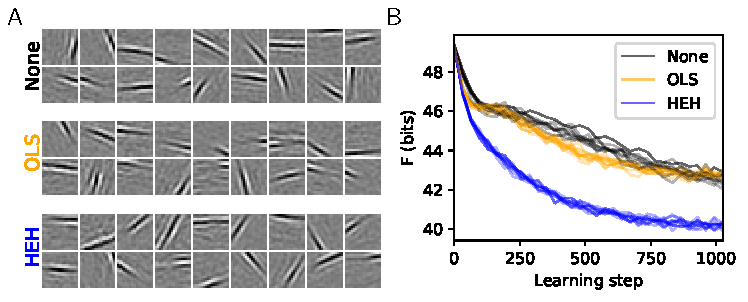
\includegraphics[width=\linewidth]{figure_map}}
\caption{
{\bf Role of homeostasis in learning sparse representations}:
We show the results of Sparse Hebbian Learning using different homeostasis algorithms at convergence ($1024$ learning steps). The compared algorithms are \texttt{None} a simple normalization of the atoms, \texttt{OLS} the method of~\citep{Olshausen97}, \texttt{HEH} the optimal homeostasis described in this paper. {\sf (A)} For each algorithm, we show $10$ randomly drawn atoms from the $324$ filters of the same size as the image patches ($16 \times 16$, $M=256$) are presented in a matrix (separated by a white border). Note that their position in the matrix is arbitrary as in ICA. {\sf (B)} Evolution of free-energy (in bits) as a function of the number of iterations. %
\label{fig:map}}%
\end{figure}%
%%------------------------------%
In particular, a component often ignored in this type of learning is the set of homeostasis mechanisms that control the average coding activity during learning. Indeed, these are implemented in the original algorithms~\citep{Olshausen97} as a heuristic that simply prevents the algorithm from diverging. It consists in most unsupervised learning algorithms simply in an equalization of the energy of each component of the dictionary~\citep{Mairal11}. However, the neural mechanisms of homeostasis are at work in many components of the neural code and are essential to the overall transduction of neural information. For example, the networks of GABA-type inhibitory neurons make it possible to regulate the overall activity of neural populations. % (citation needed). 
This mechanism then makes it possible to balance the contribution of the excitatory populations with respect to that in inhibitory populations. By this mechanism, this type of so-called balanced networks can explain many features inherent in the primary visual cortex~\citep{Hansel12}. These mechanisms, which often take the form of normalization rules~\citep{Schwartz01} in the network, are often used as normative theory to explain the mechanisms present in the primary visual cortex~\citep{Carandini12}. However, this work is often intended to show that the cells' selectivity that emerges from these algorithms have the same characteristics as that observed in neurophysiology~\citep{Ringach02,Rehn07, Loxley17}. Other algorithms use nonlinearities that implicitly implement homeostatic rules in neuro-mimetic algorithms~\citep{Brito16}. These non-linearities are mainly used in the output of successive layers of deep learning networks that are nowadays widely used for image classification or artificial intelligence. However most of these non-linear normalization rules are based on heuristics mimicking neural mechanisms but are not justified as part of the global problem of unsupervised learning. Framing this problem in a probabilistic framework allows to consider in addition to coding and learning the intermediate time scale of homeostasis. This allows us also to associate homeostasis with adaptation mechanisms~\citep{Rao99}. Our main argument is that by optimizing unsupervised learning at different time scales, we allow for the implementation of fast algorithms compatible with the performance of biological networks and in comparison with classical~\citep{Olshausen97} or Deep Learning approaches.

%: outline
This paper is organized according to the following plan. First we will define a simple algorithm for controlling the selection of coefficients in sparse coding algorithms based on a set of non-linear functions similar to neural gain normalization mechanisms. Such functions will be used to implement an homeostasis mechanism based on histogram equalization by progressively adapting these non-linear functions. %We will derive an optimal rule for homeostatic adaptation based on histogram equalization. 
Second, we will then show quantitative results of this optimal algorithm by applying it to different pairs of coding and learning algorithms. %By using different learning databases, we will be able to give a quantitative analysis that will make it possible to compare these different solutions. 
In addition, we will propose a simplification of this homeostasis algorithm based on the activation probability and show that it yields similar quantitative results.
%: scripts on github
All these algorithms were implemented using using \verb+Python+ (version 3.6.5)
with packages \verb+NumPy+ (version 1.14.3), \verb+sklearn+ (version 0.19.1) and \verb+SciPy+ (version 1.1.0)~\citep{Oliphant07}.
%on a cluster of Linux computing nodes.
%Visualization was performed using \verb+Matplotlib+ (version 2.2.2)~\citep{Hunter07}.
In particular, we focused in our architecture to be able to quantitatively cross-validate for every single hyper-parameters\footnote{These python scripts are available at \url{https://github.com/XXX/ZZZ}. % and documented at \url{https://pythonhosted.org/ZZZ}.
}. %Indeed, we think it is better to spend time on this than to have only one model with zillions of parameters that is optimized once.
%Such an algorithmic framework is implemented in the SHL-scripts package\footnote{These scripts are available at~\url{https://github.com/bicv/SHL_scripts} and documented at~\url{https://pythonhosted.org/SHL_scripts}.}.
%These scripts allow the retrieval of the database of natural images and the replication of the results of~\citep{Perrinet10shl} reported in this section.
To simplify the optimal rule of homeostasis, we will then deliver a neuro-mimetic homeostasis algorithm derived from the optimal rule by using a simple heuristic. We will then compare the results of this new algorithm with the optimal algorithm as well as with other existing unsupervised learning algorithms~\citep{Olshausen97, Sandin17}.
% ----------------------------------------------------------------------
\section{Unsupervised learning and the optimal representation of images}%\label{algorithm}
% ----------------------------------------------------------------------
% - noise comes from independent mixings (Cournot) - inversely, knowing the mixes, we extract the signal
% - we wish to reduce noise as much as possible by having the least number of sources => sparse coding (inverse of central limit theorem?)
% Link with VAE : https://wiseodd.github.io/techblog/2016/12/10/variational-autoencoder/
%- encoder / decoder
%- variational auto-encoder
%- sensory error versus prediction error
%
%: free-energy formulation
Visual items composing natural images are often sparse, such that knowing a model for the generation of images, the brain may use this property to reconstruct images with only a few of these items. 
In the context of the representation of natural images\footnote{We use image patches drawn from large images of outdoor scenes, as provided in the \emph{kodakdb} database which is available in the code's repository.} $\image = (\image_k)_{k=1}^L \in \RR^{L \times M}$ represented as a set of $L$ vector samples as images raveled along $M$ pixels (the $\image_{j, k} \in \RR$ are the corresponding luminance values), let us assume the generic Generative Linear Model, such that $\image = \dico \coef + \epsilon $, where by definition, the coefficients are denoted by $\coef = (\coef_k)_{k=1}^L \in \RR^{L \times N}$ and the dictionary by $\dico \in \RR^{N \times M}$. Finally, $\epsilon \in \RR^{L \times M}$ is a Gaussian iid noise which is Normal without loss of generality by scaling the norm of the dictionary's rows. Knowing this model, unsupervised learning aims at finding the least surprising causes (the parameters $\coef$ and $\dico$) for the data $\image$ but also the fact that we may only have access to a (possibly wrong) recognition model $q_\Psi(\coef | \image_k)$ for any sample $k$ (where $\Psi$ are the parameters of this model) to encode the image into coefficients. In probabilistic term, this amounts to minimize the free-energy $F$ as a bound on surprise of the (unknown) density of the parameters $p_\dico( \coef | \image_k)$~\citep{Friston12,Kingma13,Doersch2016}:
\begin{equation} -\log p_\dico( \coef | \image_k) \leq F \eqdef KL( q_\Psi(\coef | \image_k) || p_\dico( \coef | \image_k) )  -\log p_\dico( \coef | \image_k) \end{equation}
where the first term in the RHS is the (positive) Kullback-Leibler distance between the density of images using the current estimate of the (unknown) marginal posterior probability.

An advantage of this formulation is that the free-energy can be rewritten as
\begin{equation} F = KL( q_\Psi(\coef | \image_k) || p_\dico(\coef) ) - \int \log p_\dico(\image_k | \coef ) dq_\Psi(\coef | \image_k) \end{equation}
In particular, using a known coding $\hat{\coef}$ of the image $\image_k$, we may approximate the free-energy by ignoring the first term in the RHS:
\begin{equation} F \approx - \log [ p(\image | \hat{\coef}, \dico ) P(\hat{\coef}) ] = \frac{1}{2} \norm{\image_k - \dico \hat{\coef}}_2^2 - \log p_\dico(\hat{\coef}) \label{eq:sparse_cost} \end{equation}
% https://github.com/bicv/Perrinet2015BICV_sparse/blob/master/sparse.tex#L374
Such hypothesis allows to retrieve the cost that is optimized in most of existing models of unsupervised learning. Explicitly, the representation is optimized by minimizing a cost defined on prior assumptions on representation's sparseness, that is on $\log p_\dico( \coef )$. For instance, learning is accomplished in {\sc SparseNet}~\citep{Olshausen97} by defining a sparse prior probability distribution function for each coefficients in the factorial form $\log p_\dico(\coef) \sim -\beta \sum_i \log ( 1 + \frac{a_i^2}{\sigma^2} )$ where $\beta$ corresponds to the steepness of the prior and $\sigma$ to its scaling (see Figure 13.2 from~\citep{Olshausen02}). Then, knowing this sparse solution, learning is defined as slowly changing the dictionary using Hebbian learning.
Indeed, performing a gradient descent on $F$ with respect to $\dico$, we have $\forall i$:
$$ \frac{\partial }{\partial \dico_i } F = \frac{1}{2} \frac{\partial }{\partial \dico_i }[(\image_k - \dico \hat{\coef})^T (\image_k - \dico \hat{\coef})] = \hat{\coef} (\image_k - \dico \hat{\coef}).$$
Similarly to Eq.~17 in~\citep{Olshausen97} or to Eq.~2 in~\citep{Smith06}, the relation is a linear ``Hebbian'' rule~\citep{Hebb49} since it enhances the weight of neurons proportionally to the correlation between pre- and post-synaptic neurons. Note that there is no learning for non-activated coefficients. The novelty of this formulation compared to other linear Hebbian learning rule such as~\citep{Oja82} is to take advantage of the sparse representation, hence the name Sparse Hebbian Learning (SHL).
%TODO say we use ADAM eta scheduling + initialization of the weights to 1/f noise (see annex)
%It is linear (at the single neuraon level) but the sparse code is not linear (at population level) \textendash link with back-propagation
In general, the parameterization of the prior in~\seeEq{sparse_cost} has major impacts on results of the sparse coding and thus on the emergence of edge-like receptive fields and requires proper tuning. For instance, a L2-norm penalty term (that is, a Gaussian prior on the coefficients) corresponds to Tikhonov regularization~\citep{Tikhonov77} and a L1-norm term (that is, an exponential prior for the coefficients) corresponds to the convex cost which is optimized by the Lasso, least-angle regression (LARS), Basis Pursuit, Fista or coordinate descent algorithms. %In fact, the definition of the prior corresponds to an objective sparseness and does not always fit to the observed probability distribution function of the coefficients. 
This is the classical formulation from~\citet{Olshausen97} but thanks to the free-energy formulation,  we have highlighted here the different hypothesis and approximation made to derive the learning rule. In particular the objective is only valid at convergence when the recognition model matches the true prior distribution of coefficients (that is, when $KL( q_\Psi(\coef | \image_k) || p_\dico(\coef) )=0$) and this approximation may influence the predicted optimal representation at convergence andfollowing the learning process.%- a nice move would be to use free-energy as a bound on surprise - and that homeostasis comes as a additional mechanism - restricts the set of possible dictionaries. (for a review, see~\citep{Pece02}) such as numerical optimization~\citep{Olshausen97}, non-negative matrix factorization~\citep{Lee99,Ranzato07} or Matching Pursuit~\citep{Perrinet03ieee,Smith06,Rehn07,Perrinet10shl}
%link of sparse coding with the cortical architecture (see rao and ballard) : 

%~~~~~~~~~~~~~~~~~~~~~~~~~~~~~~~~~~~%
\subsection{Algorithm: Sparse Coding with a control mechanism for the selection of atoms}
% TODO: check when we use 'atoms' or 'components'
%~~~~~~~~~~~~~~~~~~~~~~~~~~~~~~~~~~~%
In fact, the spiking nature of neural information demonstrates that the transition from an inactive to an active state is far more significant at the coding time scale than smooth changes of the firing rate. 
This is for instance perfectly illustrated by the binary nature of the neural code in the auditory cortex of rats~\citep{DeWeese03}. Binary codes also emerge as optimal neural codes for rapid signal transmission~\citep{Bethge03}. This is also relevant for neuromorphic systems which transmit discrete, asynchronous events (such as a network packet). With a binary event-based code, the cost is only incremented when a new neuron gets active, regardless to the analog value. Stating that an active neuron carries a bounded amount of information of $\lambda$ bits, an upper bound for the representation cost of neural activity on the receiver end is proportional to the count of active neurons, that is, to the $\ell_0$ pseudo-norm $\norm{\coef}_0 = \abs{\enscond{i}{\coef_i \neq 0}}$:%
\begin{equation}%
F \approx  \frac{1}{2} \norm{\image_k - \dico \coef}_2^2 + \lambda\norm{\coef}_0%
\label{eq:L0_cost}%
\end{equation}%
This cost is similar with information criteria such as the Akaike Information Criteria~\citep{Akaike74} or distortion rate~\citep[p.~571]{Mallat98}. For $\lambda=\log_2 N$, it gives the total information (in bits) to code for the residual (using entropic coding) and the list of spikes' addresses. In general, the high inter-connectivity of neurons (on average $10000$ synapses per neurons) justifies such an informational perspective with respect to the analog quantization of information in the point-to-point transfer of information between neurons. 
However, \seeEq{L0_cost} defines a harder cost to optimize (in comparison to convex formulations in Equation~\ref{eq:sparse_cost} for instance) since the hard $\ell_0$ pseudo-norm sparseness leads to a non-convex optimization problem which is \emph{NP-complete} with respect to the dimension $M$ of the dictionary~\citep[p.~418]{Mallat98}.
%The different SHL algorithms simply differ by the coding step.
%This implies that they only differ by first, how sparseness is defined at a functional level and second, how the inverse problem corresponding to the coding step is solved at the algorithmic level.
%Most of the schemes cited above use a less strict, parametric definition of sparseness (like the convex L$_1$-norm), but for which a mathematical formulation of the optimization problem exists.
%Few studies such as~\citep{Liu14,Peharz12} use the stricter $\ell_0$ pseudo-norm as the coding problem gets more difficult.
%A thorough comparison of these different strategies was recently presented in~\citep{Charles12}.
%See also~\citep{Aharon06} for properties of the coding solutions to the $\ell_0$ pseudo-norm.
%Similarly, in~\citep{Perrinet10shl}, we preferred to retrieve an approximate solution to the coding problem to have a better match with the measure of efficiency~\seeEq{L0_cost}. % (see Section~\ref{sec:matchingpursuit} for a description of the algorithm)

Still, there are many solutions to this optimization problem and here, we will use a generalized version of the {\color{BrickRed}matching} {\color{OliveGreen}pursuit} algorithm~\citep[p.~XXX]{Mallat98}. A crucial aspect of this algorithm is the $\ArgMax$ function as it produces at each step a competition among $N$ neurons. For this reason, we will introduce a mechanism to tune this competition. For any signal $\image_k$ drawn from the database:%~\citep{Mallat93}:
%\begin{equation} \hat{\coef}= \Arg\Max \end{equation}
\begin{enumerate}%

	\item set the sparse vector $\coef$ to zero,
	\item initialize $\bar{\coef}_i=<\image_k, \dico_i >$ for all $i$,% using~\seeEq{coco},%N
	\item while $\norm{\coef}_0<N_0$:
	\begin{enumerate}
		{\color{BrickRed}
			\item select the best match: $i^\ast = \ArgMax_{i} [z_i( \bar{\coef}_i )]$,% with~\seeEq{mp1},
		\item set the sparse coefficient: $\coef_{i^\ast} = \bar{\coef}_{i^\ast}$,
		}
		{\color{OliveGreen}\item update residual coefficients: $\forall i, \bar{\coef}_i \leftarrow \bar{\coef}_i - \coef_{i^\ast} <\dico_{i^\ast} , \dico_i > $,% for all $i$ using~\seeEq{mp3},
}
	\end{enumerate}
\end{enumerate}
Where the parameter $N_0>0$ controls the amount of sparsity that we impose to the coding. The novelty of this algorithm presented here lies in the scalar functions $z_i$ which control the competition for the best match between components in the algorithm. While in the original algorithm an identical symmetric function is chosen (that is, $\forall i, z_i(\coef) = |\coef|$), we will define at first this functions as the non-linear rectified linear unit (ReLU) with gain $\gamma_i$: $\forall i, z_i (\coef_i) = \gamma_i * \coef_i * \delta(\coef_i>0)$ and $\delta$ is Kronecker's indicator function. 
%It is at this point important to note that in this algorithm,
%we achieve an exponential convergence of the squared error~\citep[p.~422]{Mallat98},
%but also that this curve can be directly derived from the coefficients' values.
%Indeed, for $N$ coefficients (that is, $\| \coef \|_0 = N$), we have the squared error equal to:
%\begin{equation}%
%E_N \eqdef \| \image - \dico\coef \| ^2 / \| \image \| ^2 = 1 - \sum_{1\leq k\leq N} a_{k}^2 / \| \image \| ^2%
%\label{eq:error}%
%\end{equation}%
%As a consequence, the sparser the distributions of coefficients, then quicker is the decrease of the residual energy.
%%Note that the observed distribution of coefficients follow a power-law. This was already observed in~\citep{Perrinet03ieee}. This power-law (``scale-free'') distribution is defined by
%%\begin{equation}%
%%\log p(a) \propto - \gamma \log a_{k}%
%%\label{eq:powerlaw}%
%%\end{equation}%
%%The value of $\gamma$ quantifies therefore the strength of the sparseness in the signal.
%% TODO: discuss this? or say it will be discussed below
%In the following section, we will describe different variations of this algorithm. To compare their respective efficiency,
%we will plot the decrease of the coefficients along with the decrease of the residual's energy. % as a measure of sparseness.
%Using such tools, we will now explore if such a property extends to full-scale images and not only to image patches,
%an important condition for using sparse models in computer vision algorithms.
%% and we will explore this aspect in the following
%%

% method zero = just normalizing the coefficitents (Mairal) 
We found that by using an algorithm like Matching Pursuit (that is using the symmetric function or setting $\forall i, \gamma_i=1$ as in~\citep{Mairal11} for instance), the learning algorithm could provide results similar to {\sc SparseNet}, but without the need of parametric assumptions on the prior by using this more generic $\ell_0$ norm sparseness. However, we observed that this class of algorithms could lead to solutions corresponding to a local minimum of the objective function: Some solutions seem as efficient as others for representing the signal but do not represent edge-like features homogeneously (\seeFig{map}-A, \texttt{None}). %  With a correct tuning of parameters, we observed that different coding schemes show qualitatively a similar emergence of edge-like filters. The specific coding algorithm used to obtain this sparseness appears to be of secondary importance as long as it is adapted to the data and yields sufficiently efficient sparse representation vectors. However, resulting dictionaries vary qualitatively among these schemes and it was unclear which algorithm is the most efficient and what was the individual role of the different mechanisms that constitute SHL schemes. At the learning level, we have shown that the homeostasis mechanism had a great influence on the qualitative distribution of learned filters~\citep{Perrinet10shl}.~\citep{Perrinet10shl}
Moreover, using the implemented sparse coding algorithms part of the \verb+sklearn+ library, we compared the convergence of the learning with different sparse coding algorithms. In particular we compared the learning as implemented with matching pursuit to that with orthogonal matching pursuit (OMP), LARS or coordinate descent (see Annex). 
In particular, for all these sparse coding algorithms, during the early learning phase, some cells may learn ``faster'' than others. There is the need for a homeostasis mechanism that will ensure convergence of learning. The goal of this work is to study the specific role of homeostasis in learning sparse representations and to propose a homeostasis mechanism based on the functions $z_i$ which optimizes the learning of an efficient representation.%
%~~~~~~~~~~~~~~~~~~~~~~~~~~~~~~~~~~~~~~~~~~~~~~~~~~~~%
\subsection{Algorithm: Histogram Equalization Homeostasis}\label{HEH}
%~~~~~~~~~~~~~~~~~~~~~~~~~~~~~~~~~~~~~~~~~~~~~~~~~~~~%
% - a measure is that the Orientation Selectivity (OS) is highest - because we know that the structure of the world is like this...
% - goals = memory / separation / representation
% we know that during learning, there are distortions in the code / dictionary : normalisation is not enough.
Knowing a dictionary and a sparse coding algorithm, we may transform any data sample $\image_k$ into a set of sparse coefficients using the above algorithm: $\coef = S(\image_k; \dico, z_i)$. As we have seen, we may use different transformation functions $z_i$ to influence the choice of coefficients such that we may use these functions to optimize an objective cost on their distribution. 
In particular, at any step \emph{during} learning, dictionaries may not have homogeneously been learnt and may exhibit different distributions. But in general, this operation may be also feasible for any other representation dictionary.
As we have seen above, a component of the free-energy is $KL( q_\Psi(\coef | \image_k) || p_\dico(\coef) )$ which gets minimal over a set of samples only when the recognition model gets closer to the true generative model. While the latter is hidden, we know about its structure in an optimal representation within a population of sensory neurons. For the particular $\ell_0$ norm sparseness, we show that sparseness is optimal, in term of Shannon entropy, when average activity within the neural population is uniformly balanced (i.e. each neuron is selected with the same probability when encoding a large set of data). 
In particular, a necessary condition for minimizing this cost is that the a priori probability of selecting coefficients are identical $\forall (i,j), q_\Psi(\coef_i)=q_\Psi(\coef_j)$ to ensure the optimality of the choice of the pseudo $\ell_0$-norm and compare it to the representation in the primary visual cortex. 
% mutual information $KL( q_\Psi(\coef | \image_k) \leq MI( q_\Psi(\coef)$%

%: % using cumulative distribution = "inverse transform sampling" / circular problem= has to be done progressively
% a monotonic point scalar function does not change the KL distance / free-energy
To achieve this uniformity, we may define an homeostatic gain control mechanism based on histogram equalization, that is, by transforming coefficients in terms of z-scores $z_i(a_i) = P( \cdot > a_i)$. Such a transform is similar to the inverse transform sampling which is used to optimize representation in auto-encoders~\citep{Ranzatto}.
Moreover, it has been found that such an adaptation mechanism is observed in the response of the retina to various contrast distributions~\citep{Laughlin81}. However, an important point is that this joint optimization problem is circular as we can not access the true posterior $p_\dico(\coef)$: Indeed, the coefficients depend on non-linear coefficients through $\coef = S(\image_k; \dico, z_i)$, while the non-linear functions depend on the (cumulative) distribution of the coefficients.
We will make the assumption that such a problem can be solved iteratively by slowly learning the non-linear functions. 
% TODO: finish "Starting ..."
Finally, the function $z_i$ for each coefficient of the sparse vector is calculated using an iterative moving average scheme (parameterized by time constant $1/\eta_h$) to smooth its evolution during learning. At the coding level, this z-score function is incorporated in the matching step of the matching pursuit algorithm, to modulate the choice of the most as that with the maximal z-score: $i^\ast = \ArgMax_i z_i(a_i)$. The rest of the algorithm is left unchanged.
We will coin this algorithm variant as Histogram Equalization Homeostasis (\texttt{HEH}). 

Furthermore, as we adapt the dictionaries progressively during Sparse Hebbian Learning, we may incorporate this \texttt{HEH} homeostasis during learning by chosing an appropriate learning rate $\eta_h$. 
To recapitulate the different choices we made from the learning to the coding and the homeostasis, the unsupervised learning can be summarized using the following steps:
The proposed algorithm is:
\begin{enumerate}%
\item Initialize the point non-linear gain functions $z_i$ to similar cumulative distribution functions and the components $\dico_i$ to random points on the unit $L$-dimensional sphere,%
\item repeat until learning converged:%
\begin{enumerate}
\item draw a signal $\image_k$ from the database,%
\item compute sparse representation vector $\coef = S(\image_k; \Psi=\{\dico, z_i, N0\})$
\item modify dictionary: $\forall i, \dico_{i} \leftarrow \dico_{i} + \eta a_{i} (\image_k - \dico\coef)$,% using~\seeEq{learn},
\item normalize dictionary: $\dico_{i} \leftarrow \dico_{i} / \norm{\dico_{i}}$,% using~\seeEq{learn},
{\color{MidnightBlue}
\item update homeostasis functions: $z_i( \cdot ) \leftarrow (1- \eta_h ) z_i( \cdot ) + \eta_h \delta( a_i \leq \cdot)$.% using~\seeEq{learn_homeo}
}
\end{enumerate}
\end{enumerate}

We compared qualitatively the set $\dico$ of receptive filters generated with different homeostasis algorithms (see Fig.~\ref{fig:map}-A). A more quantitative study of the coding is shown by comparing the decrease of free-energy as a function of the iteration step (see Fig.~\ref{fig:map}-B). This demonstrate that forcing the learning activity to be uniformly spread among all receptive fields results in a faster convergence of the representation error as represented by the decrease of free-energy.
%------------------------------%
%: see Figure~\ref{fig:HEH}
\begin{figure}[!ht]%%[p!]
\centering{
\begin{tikzpicture}
%\draw [anchor=north west] (0, .8\linewidth) node {\includegraphics[width=\linewidth]{PDF_nohomeo}};
%\draw [anchor=north west] (0, .4\linewidth) node {\includegraphics[width=\linewidth]{z_score}};
%\draw [anchor=north west] (0, .0) node {\includegraphics[width=\linewidth]{PDF_homeo}};
\draw (.7\linewidth, 0) node [above right=0mm] {$\mathsf{A}$};
\draw (.3\linewidth, 0) node [above right=0mm] {$\mathsf{B}$};
\draw (-.1\linewidth, 0) node [above right=0mm] {$\mathsf{C}$};
\draw (.0\linewidth, .38\linewidth) node [above right=0mm] {$\mathsf{box}$};
\draw (.85\linewidth, .38\linewidth) node [above right=0mm] {$\mathsf{box}$};
\end{tikzpicture}}
\caption{
{\bf Optimal homeostasis and its role in unsupervised learning}:
{\sf (A)}~~Non-linear homeostatic functions $z_i, \forall i$ learned using Hebbian learning. These functions were computed for different homeostatic strategies (\texttt{None}, \texttt{OLS} or \texttt{HEH}) but only used in \texttt{HEH}. At convergence of \texttt{HEH}, the probability of choosing any filter is independent. As a result, entropy is maximal, a property which is essential for the optimal representation of signals in distributed networks such as the brain.
{\sf (B)}~Effect of learning rate $\eta$ on the final cost as computed for the same learning algorithms but with different homeostatic strategies (\texttt{None}, \texttt{OLS} or \texttt{HEH}).
{\sf (C)}~Effect of homeostatic learning rate $\eta_h$ on the final cost. This shows that \texttt{HEH} is robust across a wide range of parameters.
%We show the results of Sparse Coding using the two different homeostasis algorithms using surrogate data where each filter was equiprobable but for which we manipulated the first half of the coefficients to be artificially twice as big. %
%{\sf (A)}~Such a situation replicates a situation arising during learning when a sub-group of filters is more active, e.~g. because it learned more salient features. Here, we show the probability of the selection of the different filters (normalized to an average of $1$) which shows a bias of the standard Matching Pursuit to select more often filters whose activity is higher. %We evaluated the efficiency of retrieving the correct coefficients to about $\ %
%{\sf (B)}~Non-linear homeostatic functions learned using Hebbian learning. These functions were initialized as the cumulative distribution function of uniform random variables. Then they are used to modify choices in the Matching step of the Matching Pursuit algorithm. Progressively, the non-linear functions converge to the (hidden) cumulative distributions of the coefficients of the surrogate, clearly showing the group of filters with twice a big coefficients.
% {\sf (C)}~At convergence, the probability of choosing any filter is uniform. As a result, entropy is maximal, a property which is essential for the optimal representation of signals in distributed networks such as the brain.
\label{fig:HEH}}%
\end{figure}%
%------------------------------%
%----------------------------------------------------------------------------%
\section{Results: Fast unsupervised learning using homeostasis}\label{results}
%----------------------------------------------------------------------------%
%\subsection{Algorithm: Approximate homeostasis}\label{HAP}
%: incompatible with nueromimetic / fast implementation
%- first method = Olshausen's homeostasis that is a gradient descent on the variance of coefficients. serves as a control
% (\seeFig{map}-A, \texttt{OLS})
We have shown above that we can find an exact solution to the problem of homeostasis during sparse hebbian learning. However, this solution has several drawbacks. First, it is computationally intensive on a conventional computer as it necessitates to store each $z_i$ function to store the cumulative distribution of each coefficient. More importantly, it seems that biological neurons seem to rather use a simple gain control mechanism. This can be used by modifying the gain of the slope of the ReLu function to operate a gradient descent on cost based on the distribution of the coefficients. For instance, the strategy of~\citep{Olshausen97} assumes a cost on the the difference between the observed variance of coefficients $V_i$ as computed over a set of samples compared to a desired value $\sigma_g$ (and assuming a multiplicative noise parametrized by $\alpha$) :
\begin{equation}%
V_i \leftarrow (1- \eta_h ) V_i + \eta_h \cdot 1/L\sum_{k=1\cdots L} a_{i, k}^2 \textrm{ and }
\gamma_i \leftarrow (1- \eta_h ) \gamma_i \cdot \left( \frac{V_i}{\sigma_g^2} \right)^\alpha
\end{equation}%
This is similar to the mechanisms of gain normalization proposed by~\citep{Schwartz01} and which were recently shown to provide efficient coding mechanisms by Simoncelli. However, compared to these methods which manipulate the gain of dictionaries based on the energy of coefficients, we propose to rather use a methodology based on the probability of activation. Indeed, the main distortion that occurs during learning is on the higher statistical moments, for instance when an atom is winning more at the earlier iterations, its pdf will typically be more kurtotic than a filter that has learned less.
%TODO say that in these variants this replaces 2e in the learning

%: Comparison to Sandin
Recently, such an approach was proposed by~\citet{Sandin17}. Based on the same observations, authors propose to optimise the coding during learning by modulating the gain of each dictionary element based on the recent history. They base their Equalitarian Matching Pursuit (\texttt{EMP}) algorithm on a heuristics which cancels the activation of all filters that were more often activated than a given threshold (parameterized by $1+\alpha_h$). In our setting, we may compute a similar algorithm using an evaluation of probability of activation followed by binary gates:
\begin{equation}%
p_i \leftarrow (1- \eta_h ) p_i + \eta_h \cdot 1/L\sum_{k=1\cdots L} (a_{i, k} > 0) \textrm{ and }
\gamma_i = \delta (p_i < N_0/N*(1+\alpha_h)
\end{equation}%
Interestingly, they reported that such a simple heuristic could improve the learning, deriving a similar result as we have shown in~\seeFig{map}. Moreover they have shown that such a homeostatic mechanism is more important than optimizing the coding algorithm, for instance by using OMP instead of MP.

%: derivation
Similarly, we may derive an approximate homeostasis algorithm based on the current activation probability but using a gradient descent approach on gain modulation. Ideally, this corresponds to finding $\gamma_i$ such that XXX. However, the sparse coding function $S(\image)$ is not derivable, yet we may use XXX
For this we need to derivate the change of modulation gain that would be necessary to achieve an equiprobable probability, that is when $\forall i, p_i = p_0 \eqdef N_0 / N$: % this replaces step 2 e in the learning
%      # cf. https://github.com/VictorBoutin/CHAMP/blob/caa2a77cc65d0043db1aeb11eedb707633a93df4/CHAMP/CHAMP_Layer.py#L365
%      gain = np.exp(-(1 / alpha_homeo) * (mean_measure-target))
\begin{equation}%
\gamma_i = \exp(-(p_i - p_0) / \alpha_h)
\end{equation}%
We will coin this variant of the algorithm Homeostasis on Activation Probability (\texttt{HAP}). % derivation p.56N de 2018-01-09 HULK
%\subsection{Approximate homeostasis yields similar performance}
Following these derivations, we quantitatively compared \texttt{OLS}, \texttt{EMP} and \texttt{HAP} to \texttt{HEH} (see~\seeFig{HAP}). This shows that while \texttt{EMP} outperforms \texttt{OLS}, \texttt{HAP} proves to be closer to the optimal solution given by \texttt{HEH}.
% effect of coding algorithm
In particular, we replicated in \texttt{HAP} the result of~\citet{Sandin17} that while homeostasis was essential in improving unsupervised learning, the coding algorithm (MP versus OMP) mattered relatively little.

%%------------------------------%
%: \seeFig{HAP}
\begin{figure}[!ht]%%[p!]
\centering{
\begin{tikzpicture}
%\draw [anchor=north west] (0, .39\linewidth) node {\includegraphics[width=.47\linewidth]{dico_MP}};
%\draw [anchor=north west] (.5\linewidth, .39\linewidth) node {\includegraphics[width=.47\linewidth]{dico_SN}};
%\draw [anchor=north west] (.25\linewidth, -.1\linewidth) node {\includegraphics[width=.47\linewidth]{dico_MEUL}};
%\draw [anchor=north west] (.1\linewidth, -.6\linewidth) node {\includegraphics[width=.8\linewidth]{Comparison_reconstruction}};
\draw (0, .39\linewidth) node [above right=0mm] {$\mathsf{A}$};
\draw (.5\linewidth, .39\linewidth) node [above right=0mm] {$\mathsf{B}$};
%\draw (.2\linewidth, -.16\linewidth) node [above right=0mm] {$\mathsf{C}$};
%\draw (.05\linewidth, -.67\linewidth) node [above right=0mm] {$\mathsf{D}$};
\draw (.0\linewidth, .0\linewidth) node [above right=0mm] {$\mathsf{box}$};
\draw (.85\linewidth, .0\linewidth) node [above right=0mm] {$\mathsf{box}$};
\end{tikzpicture}}
\caption{
{\bf Comparative evaluation of homeostatic strategies}: %
 {\sf (A)}~10 from the 324 dictionaries learned for the 3 algorithms (\texttt{HEH}, \texttt{EMP}, \texttt{HAP}) and compared to the simple normalisation (\texttt{None}). {\sf (B)}~Comparison of the free-energy during learning: The convergence velocity of \texttt{HAP} is slightly better as \texttt{EMP} and is similar to the more demanding HEH homeostatic, demonstrating that this could be a good compromise for fast unsupervised learning.
\label{fig:HAP}}%
%\caption{
%{\bf Quantitative role of homeostasis in a classification network}: We used the generic MNIST protocol to assess the role of the homeostasis algorithm on classification. %
% {\sf (A-C)}~144 dictionaries learned from the MNIST database with a sparseness of 5 after 10000 iterations with {\sf (A)}~MP Algorithm ($\eta=0.01$): No homeostasis regulation, only a small subset of dictionaries are selected with a high probability to describe the dataset.
%{\sf (B)}~SPARSENET Algorithm ($\eta=0.01$, $\eta_h=0.01$, $\alpha_h=0.02$): The homeostasis regulation is made by normalizing the volatility.
%{\sf (C)}~MEUL Algorithm ($\eta=0.01$, $\eta_h=0.01$): All dictionaries are selected with the same probability to describe the dataset, leading to a cooperative learning.
% {\sf (D)}~Comparison of the reconstruction error (computed as the square root of the squared difference between the image and the residual) for the 3 algorithms (MEUL, SPARSENET, MP): The convergence velocity of MEUL is higher than SPARSENET and MP.
%\label{fig:quant}}%
\end{figure}%
%%------------------------------%

%-----------------------------------------------------------------%
\section{Discussion and conclusion}\label{discussion-et-conclusion}
%-----------------------------------------------------------------%
%
% LUP\ IS\ HERE\
%
%: 2- benchmarking of computation time: toward event-driven?

% Finally, we show that such an algorithm can be extended to convolutional architectures and we show the results obtained on different natural image databases.
%
One core advantage of sparse representations is the efficient coding of complex signals using compact codes. For instance, it allows for the representation of any sample as a combination of few elements drawn from a large dictionary of basis functions. In the context of the efficient processing of natural images, we propose here that such sparse coding strategies can be optimized by designing a proper homeostatic rule regulating the competition between the elements of the dictionary. Indeed, a common design for unsupervised learning rules relies on a gradient descent over a cost measuring representation quality with respect to sparseness. The sparseness constraint introduces a competition which can be optimized by ensuring that each item in the dictionary is selected as often as others. We implemented this rule by introducing a non-linear gain normalization similar to what is observed in biological neural networks. We validated this theoretical insight by challenging this adaptive unsupervised learning algorithm with different heuristics for homeostasis. Simulations show that at convergence, while the coding accuracy did not vary much, including homeostasis changed qualitatively the learned features. In particular, homeostasis results in a more homogeneous set of orientation selective filters, which is closer to what is found in the visual cortex of mammals~\citep{Ringach02,Rehn07,Loxley17}. To further validate these results, we quantitatively compared the efficiency of the different variants of the algorithms, both at the level of homeostasis (homeostatic learning rate, parameters of the heuristics), but also to the coding (by changing $M$, $N$ or $N_0$) and to the learning (by changing the learning rate, the scheduling or $M$). This showed that overall, the neuro-inspired homeostatic algorithm provided with the best compromise between efficiency and computational cost. In summary, this biologically-inspired learning rule demonstrates that principles observed in neural computations can help improve real-life machine learning algorithms.

%2. importance of homeo - vanishing term in deep learning -> use deep learning to validate output
%3. application to asynchronous / focal log-polar (retinal) input / continuous learning / credit assignement (no access to true residual)
By developing this fast learning algorithm we hope for its rapid application in artificial intelligence algorithms. This type of architecture is economical, efficient and fast. It makes it possible to be transferred to most deep learning algorithms, a major flaw of which is to be very greedy in computing resources. In particular, we are considering perspectives for coding within a dynamic flow of sensory data and we hope to apply this type of algorithm on embedded systems such as aerial robots. Along with this, we hope that this new type of rapid unsupervised learning algorithm can provide a normative theory for the coding of information in low-level sensory processing, whether it is visual or auditory, for example. Moreover, by its nature, this algorithm can easily be extended to convolutional networks such as those used in deep learning neural networks. This extension is possible by extending the filter dictionary by the hypothesis of invariances to the translation of representations. Our results on different databases show the stable and rapid emergence of characteristic filters on these different bases (see Annex). This result shows a probable prospect of extending this representation and for which we hope to obtain classification results superior to the algorithms existing in the state-of-the-art. Finally such computational results highlight the importance of homeostasis in unsupervised learning algorithms and for the study of neural systems.
%%%%%-----------------------------------------------------------------
% NIPS submissisons are anonymous
%\section*{Acknowledgments}
%\Acknowledgments
%%%-----------------------------------------------------------------
\printbibliography

\end{document}
